\chapter{開発} 
\thispagestyle{plain}   % chapterの直後に必ず指定

本研究では,\ref{sec:minecraft}章で述べたMinecraftの特性に焦点を当て,Minecraftの中で大規模言語モデルを搭載したbotを作成し,そのbotと人間が対話を行ったり,共同作業を行ったりすることで,人間とAIの協力・協調関係の協会と可能性を探求する.

本章では作成したbotについて解説する.
システムの全体像は図\ref{fig:system}のとおりである.
プレイヤーはbotログイン用webアプリケーションを使用して,botをMinecraftのマルチサーバーに参加させることが可能である.
その後プレイヤーは,botが参加したマルチサーバーと同じサーバーにログインしMinecraftのチャットの機能(デフォルトでTキー)を用いてbotと対話することができる.

マルチサーバーにログインしたbotはプレイヤーからのチャットの情報を大規模言語モデルに送り,大規模言語モデルからの返答をもとにプレイヤーへ返答や行動を行うことが可能である.
詳細な機能については\ref{sec:webapp}節から\ref{sec:build_mode}節で解説する.

\begin{figure}[H]
    \centering
    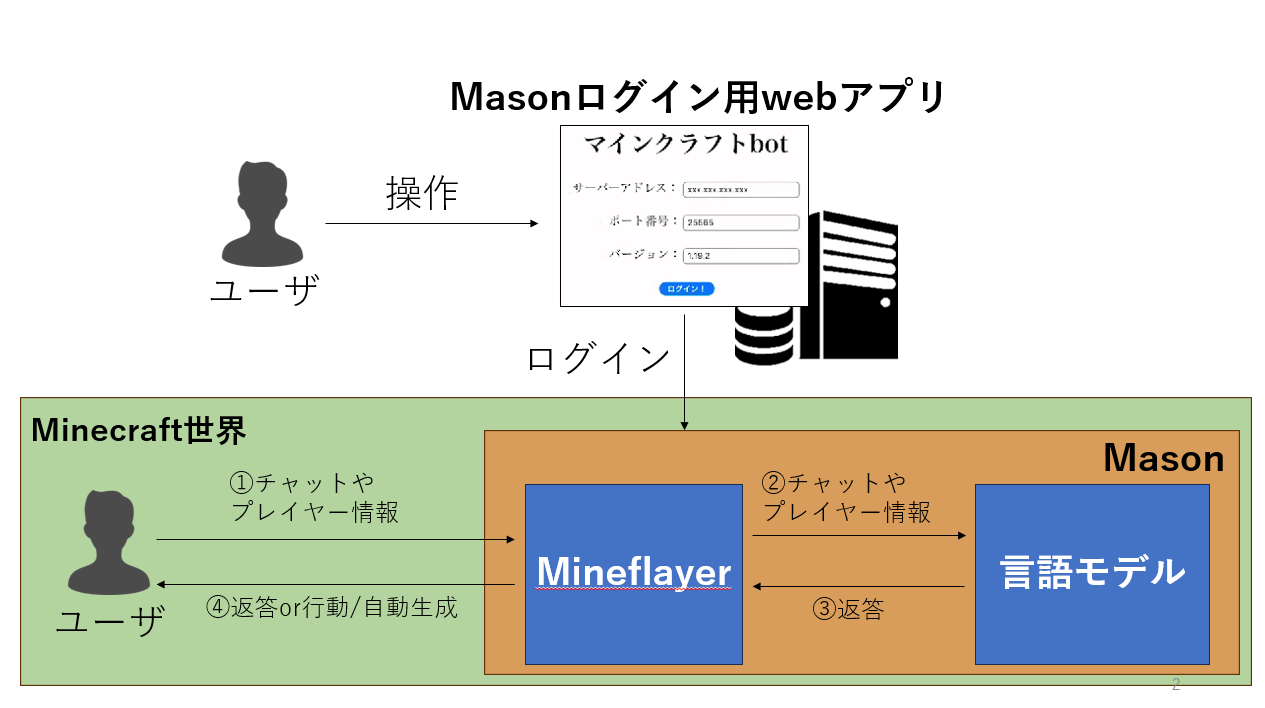
\includegraphics[width=0.8\textwidth]{fig/my_system.PNG}
    \caption{システムの概要}
    \label{fig:system}
\end{figure}

\section{Webアプリケーション}\label{sec:webapp}
人間とAIの協力・協調を主目的とする以上,ユーザビリティについて追求する必要があると考えたため,botをログインさせるためのWebアプリケーションを作成した.
従来までの方法でbotを動かすためには,プログラミング環境構築のスキルを必要とするが,このアプリケーションではマイクラのマルチにログインする時と同様の情報を入力することで,簡単にbotをログインさせることが可能となった.

\begin{figure}[H]
    \centering
    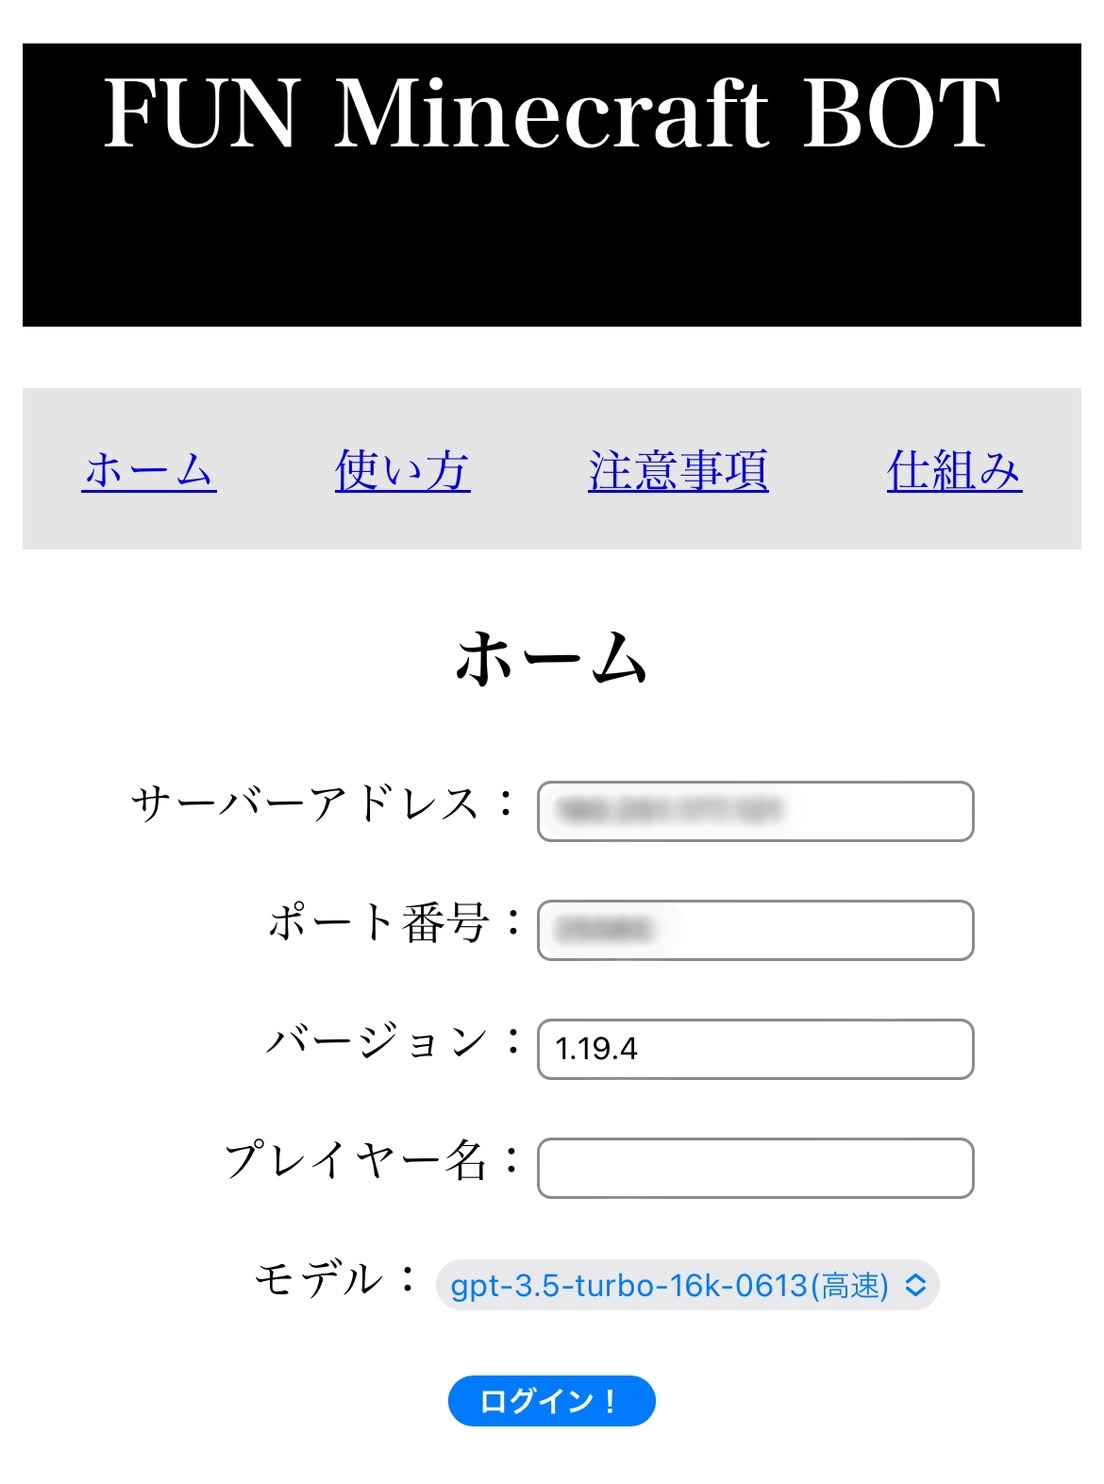
\includegraphics[width=0.5\textwidth]{fig/web_app.jpg}
    \caption{Webアプリケーションのホーム画像}
    \label{fig:web_app}
\end{figure}

\section{行動}\label{sec:act}
botがMinecraft世界に干渉して人間の作業などを手伝うことができるように,いくつかの行動を作成した.
botの各行動はMineflayer API\cite{bib:Mineflayer}を用いて実装した.
Mineflayer APIの関数は例外が発生するとbotがログアウトしてしまうため,基本的にMineflayer APIの関数に例外処理を加えて開発している.
作成した行動には表\ref{tab:action}の種類がある.

\begin{table}[H]
    \caption{行動の種類}\label{tab:action}
    \centering
    \begin{tabular}{lp{0.7\linewidth}}
        \hline \hline
        move\_to\_position & 説明: 指定した座標へ移動. \\
          & 引数: int x, int y, int z \\
        \hline
        mine\_block & 説明: nameで指定したブロックを指定個数採掘して集める. \\
          & 引数: str name, int count \\
        \hline
        smelt\_item & 説明: item\_nameで指定したアイテムをcountの個数分かまどで製錬する.fuel\_nameで燃料を指定する. \\
          & 引数: str item\_name, str fuel\_name, int count \\
        \hline
        mine\_block & 説明: nameで指定したブロックを指定個数採掘して集める \\
          & 引数: str name, int count \\
        \hline
        craft\_item & 説明: nameで指定したアイテムをcountの個数分,作業台で作成する. \\
          & 引数: str name, int count \\
        \hline
        get\_item\_chest & 説明: chest\_positionで指定した位置にあるチェストから,item\_dictのアイテムを個数分取り出す. \\
          & 引数: Vec3 chest\_position, dict[str,int] item\_dict \\
        \hline
        deposit\_item\_chest & 説明: chest\_positionで指定した位置にあるチェストに,item\_dictのアイテムを個数分入れる. \\
          & 引数: Vec3 chest\_position, dict[str,int] item\_dict \\
        \hline
        check\_item\_chest & 説明: chest\_positionで指定した位置にあるチェストのアイテムを確認する. \\
          & 引数: Vec3 chest\_position \\
        \hline
        farm & 説明: 近くの農地に所持している小麦の種を植える. \\
          & 引数: なし \\
        \hline
    \end{tabular}
\end{table}

\section{大規模言語モデルによるタスクの提示や会話}\label{sec:gpt_res}
複数の大規模言語モデルを組み合わせることによって,サバイバルモードのプレイヤー向けの対話機能を作成した.
この機能では,プレイヤーの発話と情報を元に,Masonが次のタスクを提示したり,\ref{sec:act}節の行動を起こすことでプレイヤーの作業を手伝ったり,質問や会話に返答することが可能になった.

プレイヤーの発話とは「how to make ~?」,「please craft ~.」,「please tell me next task.」のような,Masonに対する会話である.

プレイヤーの情報とは表\ref{tab:player_data}に示す,プレイヤーの現在の状態を表したJSONデータである.
\begin{table}[H]
    \caption{行動の種類}\label{tab:player_data}
    \centering
    \begin{tabular}{llp{0.6\linewidth}}
        \hline \hline
        キー & データ型 & 説明 \\
        \hline
        goals & string & プレイヤーの目標. \\
        biome & string & プレイヤーが現在居るバイオーム. \\
        time & string & Minecraft世界の現在時刻.0~23999までの値であり,13000~は夜を表す. \\
        blocks & list[string] & プレイヤーの半径10ブロック以内のブロックの種類 \\
        entities & list[string] & プレイヤーの半径10ブロック以内のエンティティの種類 \\
        health & string & プレイヤーの体力(20が最大) \\
        hunger & string & プレイヤーの満腹度(20が最大) \\
        pos & string & プレイヤーの現在の3次元座標 \\
        equip & list[string] & プレイヤーの装備中のアイテム(右手,左手,頭,体,脚,足) \\
        collected & list[string] & プレイヤーがこれまでに集めたアイテム \\
        chest & list[string] & 近くのチェスト \\
        \hline
    \end{tabular}
\end{table}

サバイバルモードのプレイヤー向けの対話機能の全体像や,プレイヤーの発話や情報の処理手順を図\ref{fig:interactive_function}に示す.
処理の手順としてまず,Chat Classificationモデルがプレイヤーの発話と情報を受け入れ,few-shot学習を使用してプレイヤーの発話を``Chat'',``Order'',``Request Next Task''の3つのカテゴリのいずれかに分類する.

発話が``Chat''に分類された場合,Chatモデルを用いて一般的な会話や質問に対応することができる.
このモデルはRetrieval-Augmented Generation (RAG)\cite{}を用いており,通常は応答することが不可能な情報に対しても,大量のデータを参考にして応答を生成することが可能である.
RAGを用いる例として,Masonのテスト環境である,FUN Minecraft Server\cite{}に関する質問などが挙げられる.
これらの情報はインターネット上に情報が少ないことからもとのGPTモデルが学習しておらず回答が不安定であるが,RAGによってMasonはそれらの特定の条件に関する質問に答えることが出来る.

発話が``Order''に分類された場合,Actionモデルを用いてMasonが命令を解釈した後,表\ref{tab:action}の行動を実行し,プレイヤーの作業を手伝うことが可能である.
Orderに分類されるプレイヤーの発話の例としては,``cut the tree''などのMasonに対する命令文が考えられる.
命令文を受け取ると,Actionモデルでは,OpenAIの関数呼び出しによって適切な関数と引数が設定され,mine\_block("oak\_log",3)のように行動を実行することが可能である.

``Request Next Task''の分類では,プレイヤーの発話や情報がNext Taskモデルに,受け渡される.
Next TaskモデルのプロンプトはVoyagerのプロンプトに基づいており,プレイヤーの発話と情報から,Masonがプレイヤーに対して次のタスクを提示する.
また,提案されたタスクはActionモデルに渡され,Actionモデルが行動を実行できる場合は,プレイヤーのタスクを支援することができる.
例えば,プレイヤー情報のcollectedのリストが空である場合,モデルはプレイヤーがまだアイテムを集めたことがなく初期状態であると推論し,Minecraftにおける最初のタスク``cut the tree''などをプレイヤーに提案する.
そして提示した``cut the tree''というタスクはActionモデルにわたり,mine\_block("oak\_log",3)といった行動を起こすことが出来る.
したがって,Masonは初期状態のプレイヤーに対して``cut the tree''というタスクを提示し,同時にMasonも木を切って作業を手伝うことが出来る.

\begin{figure}[H]
    \centering
    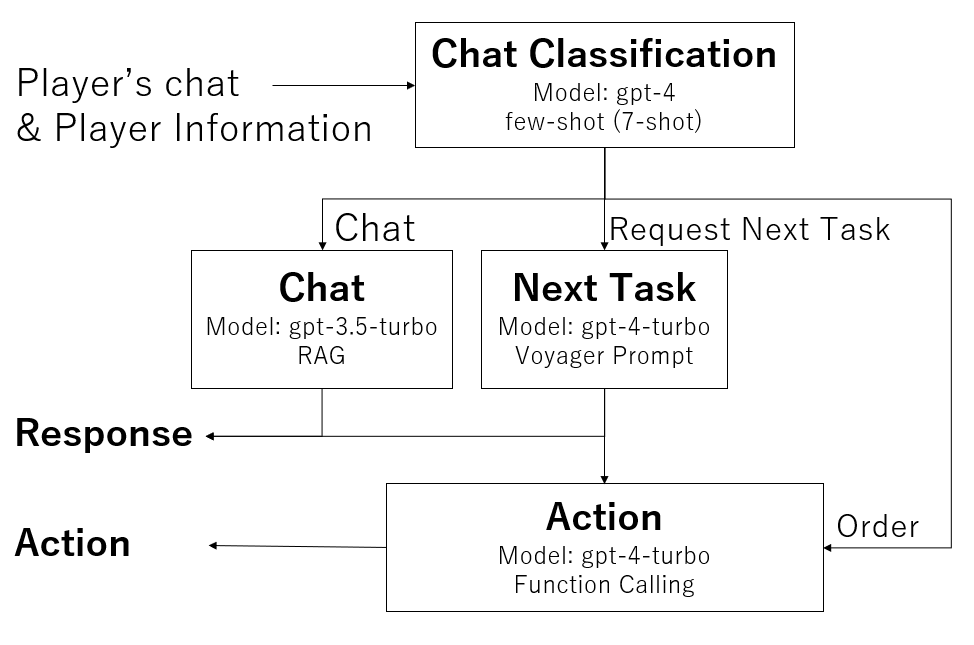
\includegraphics[width=0.8\textwidth]{fig/interactive_function.PNG}
    \caption{サバイバルモード向け対話機能の全体像}
    \label{fig:interactive_function}
\end{figure}

\section{構造物自動生成}\label{sec:build_mode}
独自のプロンプトによって,クリエイティブモードのプレイヤー向けに構造物の自動生成が可能になった.
このプロンプトには,/fillコマンドで構造物を生成すること,/fillコマンドの説明,3次元座標の概念の説明,/fillコマンドの使用例を記述した.

このプロンプトを初期プロンプトとして,作りたい構造物のプロンプトを送ると,fillコマンドのリストが提示され,fillコマンドのリストをMineflayerを通して順番に実行すると構造物が生成される.
また,追加のプロンプトを使用して装飾を追加したり,修正を加えたりすることができる.
\section{構造物自動生成のファインチューニング}
